\documentclass{article}
\usepackage[latin1]{inputenc}
\usepackage[T1]{fontenc}
\usepackage{times}
\usepackage{mathtime}
\usepackage{url}
\usepackage{amsmath}
\usepackage{alltt}
\usepackage[dvips]{graphics}
\begin{document}
 
\section{Name }
\textsc{melting} - nearest-neighbor computation of nucleic acid hybridation
\section{Synopsis}
\textbf{melting} [\textit{options }]  
\section{Description }

\textsc{melting} computes, for a nucleic acid duplex, the enthalpy and the
entropy of the helix-coil transition, and then its melting temperature. Four
types of hybridisation are possible: DNA/DNA, DNA/RNA, RNA/RNA and 2-O-Methyl RNA/RNA. The program
uses the method of nearest-neighbors. The set of thermodynamic parameters can be
easely changed, for instance following an experimental breakthrough. Melting is
a free program in both sense of the term. It comes with no cost and it is
open-source. In addition it is coded in Java (1.5) and can be compiled on any
operating system.

If you use \textsc{melting}, please quote

\begin{quote}
  Le Nov\`ere. \textsc{melting}, a free tool to compute the
    melting temperature of nucleic acid duplex. \emph{Bioinformatics}, 17: 1226-1227. 
\end{quote}

\section{Options }

The options are treated sequentially. If there is a conflict between the value
of two options, the latter normally erases the former.

\begin{description}
\subsection{Information about MELTING}

\item [\textbf{-h}]\mbox{}\\ 
  Displays a short help and quit.
\item [\textbf{-L}]\mbox{}\\ 
  Prints the legal informations and quit. 
\item [\textbf{-V}  ]\mbox{}\\ 
  Displays the version number and quit.  
\item [\textbf{-p}]\mbox{}\\ 
  Return the directory supposed to contain the sets of calorimetric parameters and quit. 
  If the environment variable NN\_PATH is set, it is returned. Otherwise, the value
  defined by default during the compilation is returned.

\subsection{Mandatory options}

\item [\textbf{-S} \textit{sequence}  ]\mbox{}\\ 
  Sequence of one strand of the nucleic 
  acid duplex, entered 5' to 3'. \textbf{Important:} 
  Uridine and thymidine are not considered as identical. The bases can be upper or lowercase.
\item [\textbf{-C} \textit{complementary\_sequence}] \mbox{}\\
  Enters the complementary sequence, from 3' to 5'. This option is mandatory if
  there are mismatches, inosine(s) or hydroxyadenine(s) between the two strands. If it is not used, the program
  will compute it as the complement of the sequence entered with the option \textbf{-S}. In case of self complementary sequences,
  The programm can automatically detect the symmetry and deduce the complementary even though there is (are) dangling
  end(s) and it is not necessary to write the complementary sequence with the option \textbf{-C}.
  Uridine and thymidine are not considered as identical. The bases can be upper or lowercase.
\item [\textbf{-E} \textit{ion1\_name=x.xxe-xx:ion2\_name=x.xxe-xx:agent1\_name=x.xxe-xx...}] \mbox{}\\
  Enters the different ion (Na, Mg, Tris, K) or agent (dNTP, DMSO, formamide) concentrations. The effect  
  of  ions and denaturing agents on  thermodynamic  stability  of nucleic  acid duplexes is complex,
  and the correcting functions are  at  best rough  approximations. All the concentrations must be positive numeric
  values and in M. There are some exceptions for the DMSO concentrations (in
  percent) and the formamide concentrations
  (in percent or M depending on the used correction method). Be aware, the $[\mbox{Tris}^+]$ is about half of the total tris buffer
  concentration.
  At least one cation concentration is mandatory, the other agents are optional. See the documentation for the concentration 
  limits. It depends on the used correction.
\item [\textbf{-P} \textit{x.xxe-xx}]\mbox{}\\ 
  Concentration of the nucleic acid strand in excess. It must be a strict positive numeric value and it is mandatory. The oligomer
  concentration is in mol/L.
\item [\textbf{-H} \textit{hybridisation\_type}]\mbox{}\\
  Specifies the hybridisation type. Moreover this parameter determines the nature of the sequences entered by the user.
  Possible values are :
  \begin{itemize}
  \item [\textit{dnadna}] : DNA sequence (option \textbf{-S}) and DNA complementary sequence (option \textbf{-C})
  \item [\textit{rnarna}] : RNA sequence (option \textbf{-S}) and RNA complementary sequence (option \textbf{-C})
  \item [\textit{dnarna}] : DNA sequence (option \textbf{-S}) and RNA complementary sequence (option \textbf{-C})
  \item [\textit{rnadna}] : RNA sequence (option \textbf{-S}) and DNA complementary sequence (option \textbf{-C})
  \item [\textit{mrnarna}] : 2-o-methyl RNA sequence (option \textbf{-S}) and RNA complementary sequence (option \textbf{-C})
  \item [\textit{mrnarna}] : RNA sequence (option \textbf{-S}) and 2-o-methyl RNA complementary sequence (option \textbf{-C})
  \end{itemize}
  This option is mandatory to select the default equations and methods to use.

\subsection{General options}

\item [\textbf{-T} \textit{xxx}  ]\mbox{}\\ 
Size threshold before approximative computation. The nearest-neighbour approach 
will be used by default if the length of the sequence is inferior to this threshold,
otherwise it is the approximative approach which will be used by default.
\item [\textbf{-v}]\mbox{}\\ 
Activates the verbose mode, issuing a lot more information about the current run  (try it once 
to see if you can get something interesting).
\item [\textbf{-nnpath} \textit{folder\_pathway}]\mbox{}\\ 
  Change the default pathway (Data) where to find the default calorimetric tables (thermodynamic parameters).
  The program will look for the file in a directory specified during the installation.
  However, if an environment variable NN\_PATH is defined, melting will search in this one first.
\item [\textbf{-O} \textit{output\_file}]\mbox{}\\ 
  The output is directed to this file instead of the standard output. The name of the file must be specified.
\item [\textbf{-self}]\mbox{}\\
  To precise that the sequence entered with the option \textbf{-S} is self complementary. No complementary sequence is mandatory. 
  The program automatically can detect a self complementary sequence for perfect matching sequences or sequences with dangling ends. 
  In these cases, the option \textbf{-self} is not necessary. Otherwise we need to precise that the sequences are self complementary with this option. 
  examples: 
    
  \begin{verbatim}
  Situation 1 : The sequence ATCGCGAT is self 
                complementary. 
      
  \end{verbatim}
  
  The option \textbf{-self} is not necessary because the programm can automatically detect it.
  
  \begin{verbatim}
  Situation 2 : The sequence -TCGCGAT is self 
                complementary with a single 
		dangling end. 
      
  \end{verbatim}
    
  The option \textbf{-self} is not necessary because the programm 
  can automatically detect it.
  
  \begin{verbatim}  
  Situation 3 :  If the sequence ATCCCGAT is self 
                 complementary with a single mismatch 
		(C/C)
      
  \end{verbatim}
  		 
  The option \textbf{-self} is necessary to precise the self 
  complementarity because the programm can't detect it.
      
 \item [\textbf{-F} \textit{factor}  ]\mbox{}\\
  This is the correction factor used to modulate the effect of the nucleic acid concentration in the computation of the melting temperature. 
  See section ALGORITHM for details. If the sequences are automatically recognized as self complementary sequences or if the option \textbf{-self}
  is used, the factor correction is automatically 1. Otherwise F is 4 if the both strands are present in equivalent amount and 1 if one strand is in excess. 
  The default factor value is 4.

\subsection{Set of thermodynamic parameters and methods (models)}

By default, the approximative mode is used for oligonucleotides longer than 60 bases (the default threshold value), otherwise the nearest 
neighbor model is used. 

\item [\textbf{-am} \textit{method\_name}]\mbox{}\\ 
  Forces to use a specific approximative formula, based on G+C content. You can use one of the following :
  
  \textsc{DNA duplexes}
    \begin{itemize}
    \item [\textit{ahs01}] (from Ahsen et al. 2001)
    \item [\textit{che93}] (from Marmur, Chester and al. 1962, 1993)
    \item [\textit{che93corr}] (from Ahsen et al. 2001 and from Marmur, Chester and al. 1962, 1993)
    \item [\textit{schdot}] (Marmur-Schildkraut-Doty formula)
    \item [\textit{owe69}] (from Owen et al. 1969)
    \item [\textit{san98}] (from Santalucia et al. 1998)
    \item [\textit{wetdna91}] (from Wetmur 1991)  (by default)
    \end{itemize}
  \textsc{RNA duplexes}
    \begin{itemize}
    \item [\textit{wetrna91}] (from Wetmur 1991)  (by default)
    \end{itemize}
  \textsc{DNA/RNA duplexes}
    \begin{itemize}
    \item [\textit{wetdnarna91}] (from Wetmur 1991)  (by default)
    \end{itemize}
  If there is no formula name after the option \textbf{-am}, we will compute the melting temperature with the default approximative formula.
  This option has to be used with caution. Note that such a calcul is increasingly incorrect when the length of  the duplex 
  decreases. Moreover, it does not take into account nucleic acid concentration, which is a strong mistake.
  examples :
  
  \begin{verbatim}
   command line 1 : "-am" 
  
  \end{verbatim}	  
  if you want to force the approximative approach with the 
  default formula.
  
  \begin{verbatim}
   command line 2 : "-am ahs01" 
  \end{verbatim}
  	  
  if you want to use the approximative formula from 
  Ahsen et al. 2001.
    	
\item [\textbf{-nn} \textit{method\_name}]\mbox{}\\ 
  Forces to use a specific nearest neighbor model. You can use one of the following :
  
  \textsc{DNA duplexes}
    \begin{itemize}
    \item [\textit{all97}] (from Allawi and Santalucia 1997)
    \item [\textit{bre86}] (from Breslauer et al. 1986)
    \item [\textit{san04}] (from Santalucia 2004)  (by default)
    \item [\textit{san96}] (from Santalucia et al. 1996)
    \item [\textit{sug96}] (from Sugimoto et al 1996)
    \item [\textit{tan04}] (from Tanaka et al. 2004)		 
    \end{itemize}
  \textsc{RNA duplexes}
    \begin{itemize}
    \item [\textit{fre86}] (from Freier al. 1986)
    \item [\textit{xia98}] (from Xia et al. 1998)  (by default)		 
    \end{itemize}
  \textsc{DNA/RNA duplexes}
    \begin{itemize}
    \item [\textit{sug95}] (from Sugimoto et al. 1995)  (by default)
    \end{itemize}
  \textsc{mRNA/RNA duplexes}
    \begin{itemize}
    \item [\textit{tur06}] (from Turner et al. 2006)  (by default)
    \end{itemize}
  If there is no formula name after the option \textbf{-nn}, we will compute the melting temperature with the default nearest neighbor model. 
  Each nearest neighbor model uses a specific xml file containing the thermodynamic values. If you want to use another file, write the file name or the file pathway preceded by ':' (-nn [optionalname:optionalfile]).
  examples:
     
  \begin{verbatim}
  Command line 1 : "-nn" 
  
  \end{verbatim}
  if you want to force the nearest neighbor computation with the default model.
  
  \begin{verbatim}
  Command line 2 : "-nn tan04" 
  
  \end{verbatim}
  if you want to use the nearest neighbor model from Tanaka et al. 2004 with the 
  thermodynamic parameters in the default xml file.
  
  \begin{verbatim}
  Command line 3 : "-nn tan04:fileName" 
  
  \end{verbatim}
  if you want to use the nearest neighbor model from Tanaka et al. 2004 with the 
  thermodynamic parameters in the file fileName.
  
  \begin{verbatim}
  Command line 4 : "-nn :fileName" 
  
  \end{verbatim}
  if you want to use the default nearest neighbor model with the thermodynamic parameters in the file fileName.
  		  
\item [\textbf{-sinMM} \textit{method\_name}]\mbox{}\\ 
  Forces to use a specific nearest neighbor model to compute the contribution of single mismatch to the thermodynamic of helix-coil transition. 
  You can use one of the following :
  
  \textsc{DNA duplexes}
    \begin{itemize}
    \item [\textit{allsanpey}] (from Allawi, Santalucia and Peyret 1997, 1998 and 1999)  (by default) 
    \end{itemize}
  \textsc{RNA duplexes}
    \begin{itemize}
    \item [\textit{tur06}] (from Turner et al. 2006)
    \item [\textit{zno07}] (from Znosko et al. 2007)  (by default)
    \item [\textit{zno08}] (from Znosko et al. 2008)		 		 
    \end{itemize}
  To change the file containing the thermodynamic parameters for single mismatch computation, the same syntax as the one for the \textbf{-nn} option is used.
  Single mismatches are not taken into account by the approximative mode.
\item [\textbf{-GU} \textit{method\_name}]\mbox{}\\ 
  Forces to use a specific nearest neighbor model to compute the contribution of GU base pairs to the thermodynamic of helix-coil transition. 
  You can use one of the following :
  
  \textsc{RNA duplexes}
    \begin{itemize}
    \item [\textit{tur99}] (from Turner et al. 1999) (by default)		 		 
    \end{itemize}
  To change the file containing the thermodynamic parameters for GU base pair computation, the same syntax as the one for the \textbf{-nn} option is used.
  GU base pairs are not taken into account by the approximative mode.
\item [\textbf{-tanMM} \textit{method\_name}]\mbox{}\\ 
  Forces to use a specific nearest neighbor model to compute the contribution of tandem mismatches to the thermodynamic of helix-coil transition. 
  You can use one of the following :
  
  \textsc{DNA duplexes}
    \begin{itemize}
    \item [\textit{allsanpey}] (from Allawi, Santalucia and Peyret 1997, 1998 and 1999)  (by default) 
    \end{itemize}
  \textsc{RNA duplexes}
    \begin{itemize}
    \item [\textit{tur99}] (from Turner et al. 1999) (by default)		 		 
    \end{itemize}
  To change the file containing the thermodynamic parameters for tandem mismatch computation, the same syntax as the one for the \textbf{-nn} option is used.
  Tandem mismatches are not taken into account by the approximative mode. Note that not all the mismatched Crick's pairs have been investigated. 
\item [\textbf{-intLP} \textit{method\_name}]\mbox{}\\ 
  Forces to use a specific nearest neighbor model to compute the contribution of internal loop to the thermodynamic of helix-coil transition. 
  You can use one of the following :
  
  \textsc{DNA duplexes}
    \begin{itemize}
    \item [\textit{san04}] (from Santalucia 2004)  (by default) 
    \end{itemize}
  \textsc{RNA duplexes}
    \begin{itemize}
    \item [\textit{tur06}] (from Turner et al. 2006) (by default)
    \item [\textit{zno07}] (from Znosko et al. 2007, only for 1x2 loop)  
    \end{itemize}
  To change the file containing the thermodynamic parameters for internal loop computation, the same syntax as the one for the \textbf{-nn} option is used.
  Internal loops are not taken into account by the approximative mode.   
\item [\textbf{-sinDE} \textit{method\_name}]\mbox{}\\ 
  Forces to use a specific nearest neighbor model to compute the contribution of single dangling end to the thermodynamic of helix-coil transition. 
  You can use one of the following :
  
  \textsc{DNA duplexes}
    \begin{itemize}
    \item [\textit{bom00}] (from Bommarito et al. 2000)  (by default) 
    \item [\textit{sugdna02}] (from Sugimoto et al. 2002, only for polyA dangling ends)      
    \end{itemize}
  \textsc{RNA duplexes}
    \begin{itemize}
    \item [\textit{sugrna02}] (from Sugimoto et al. 2002, only for polyA dangling ends)
    \item [\textit{ser08}] (from Serra et al. 2008)  (by default) 		  
    \end{itemize}
  To change the file containing the thermodynamic parameters for single dangling end computation, the same syntax as the one for the \textbf{-nn} option is used.
  Single dangling ends are not taken into account by the approximative mode.   
\item [\textbf{-secDE} \textit{method\_name}]\mbox{}\\ 
  Forces to use a specific nearest neighbor model to compute the contribution of double dangling end to the thermodynamic of helix-coil transition. 
  You can use one of the following :
  
  \textsc{DNA duplexes}
    \begin{itemize}
    \item [\textit{sugdna02}] (from Sugimoto et al. 2002, only for polyA dangling ends) (by default)     
    \end{itemize}
  \textsc{RNA duplexes}
    \begin{itemize}
    \item [\textit{sugrna02}] (from Sugimoto et al. 2002, only for polyA dangling ends)
    \item [\textit{ser05}] (from Serra et al. 2005) 	
    \item [\textit{ser06}] (from Serra et al. 2006) (by default) 			 
    \end{itemize}
  To change the file containing the thermodynamic parameters for double dangling end computation, the same syntax as the one for the \textbf{-nn} option is used.
  Double dangling ends are not taken into account by the approximative mode.  
\item [\textbf{-longDE} \textit{method\_name}]\mbox{}\\ 
  Forces to use a specific nearest neighbor model to compute the contribution of long dangling end to the thermodynamic of helix-coil transition. 
  You can use one of the following :
  
  \textsc{DNA duplexes}
    \begin{itemize}
    \item [\textit{sugdna02}] (from Sugimoto et al. 2002, only for polyA dangling ends) (by default)     
    \end{itemize}
  \textsc{RNA duplexes}
    \begin{itemize}
    \item [\textit{sugrna02}] (from Sugimoto et al. 2002, only for polyA dangling ends)
    \end{itemize}
  To change the file containing the thermodynamic parameters for long dangling end computation, the same syntax as the one for the \textbf{-nn} option is used.
  Long dangling ends are not taken into account by the approximative mode.  
\item [\textbf{-sinBU} \textit{method\_name}]\mbox{}\\ 
  Forces to use a specific nearest neighbor model to compute the contribution of single bulge loop to the thermodynamic of helix-coil transition. 
  You can use one of the following :
  
  \textsc{DNA duplexes}
    \begin{itemize}
    \item [\textit{san04}] (from Santalucia 2004) 
    \item [\textit{tan04}] (from Tanaka et al. 2004)  (by default) 	    
    \end{itemize}
  \textsc{RNA duplexes}
    \begin{itemize}
    \item [\textit{ser07}] (from Serra et al. 2007)
    \item [\textit{tur06}] (from Turner et al. 1999 and 2006)  (by default) 			 			 
    \end{itemize}
  To change the file containing the thermodynamic parameters for single bulge loop computation, the same syntax as the one for the \textbf{-nn} option is used.
  Single bulge loops are not taken into account by the approximative mode. 
\item [\textbf{-lonBU} \textit{method\_name}]\mbox{}\\ 
  Forces to use a specific nearest neighbor model to compute the contribution of long bulge loop to the thermodynamic of helix-coil transition. 
  You can use one of the following :
  
  \textsc{DNA duplexes}
    \begin{itemize}
    \item [\textit{san04}] (from Santalucia 2004) (by default)
    \end{itemize}
  \textsc{RNA duplexes}
    \begin{itemize}
    \item [\textit{tur06}] (from Turner et al. 1999 and 2006)  (by default) 			 			 
    \end{itemize}
  To change the file containing the thermodynamic parameters for long bulge loop computation, the same syntax as the one for the \textbf{-nn} option is used.
  Long bulge loops are not taken into account by the approximative mode.
\item [\textbf{-CNG} \textit{method\_name}]\mbox{}\\ 
  Forces to use a specific nearest neighbor model to compute the contribution of CNG repeats to the thermodynamic of helix-coil transition.
  N represents a single mismatch of type N/N. 
  You can use one of the following :
  
  \textsc{RNA duplexes}
    \begin{itemize}
    \item [\textit{bro05}] (from Broda et al. 2005) (by default)			 			 
    \end{itemize}
  To change the file containing the thermodynamic parameters for CNG repeats computation, the same syntax as the one for the \textbf{-nn} option is used.
  CNG repeats are not taken into account by the approximative mode. 
  Be aware : Melting can compute the contribution of CNG repeats to the thermodynamic of helix-coil transition for only 2 to 7 CNG repeats.
\item [\textbf{-ino} \textit{method\_name}]\mbox{}\\ 
  Forces to use a specific nearest neighbor model to compute the contribution of inosine bases (I) to the thermodynamic of helix-coil transition. 
  You can use one of the following :
  
  \textsc{DNA duplexes}
    \begin{itemize}
    \item [\textit{san05}] (from Santalucia et al. 2005)  (by default)
    \end{itemize}
  \textsc{RNA duplexes}
    \begin{itemize}
    \item [\textit{zno07}] (from Znosco et al. 2007, only IU base pairs)  (by default)  			 			 
    \end{itemize}
  To change the file containing the thermodynamic parameters for inosine bases computation, the same syntax as the one for the \textbf{-nn} option is used.
  Inosine bases (I) are not taken into account by the approximative mode. 
\item [\textbf{-ha} \textit{method\_name}]\mbox{}\\ 
  Forces to use a specific nearest neighbor model to compute the contribution of hydroxyadenine bases (A*) to the thermodynamic of helix-coil transition. 
  You can use one of the following :
  
  \textsc{DNA duplexes}
    \begin{itemize}
    \item [\textit{sug01}] (from Sugimoto et al. 2001) (by default)
    \end{itemize}
  To change the file containing the thermodynamic parameters for hydroxyadenine bases computation, the same syntax as the one for the \textbf{-nn} option is used.
  Hydroxyadenine bases (A*) are not taken into account by the approximative mode.
\item [\textbf{-azo} \textit{method\_name}]\mbox{}\\ 
  Forces to use a specific nearest neighbor model to compute the contribution of azobenzenes (X\_T for trans azobenzenes and X\_C for cis azobenzenes) to the thermodynamic 
  of helix-coil transition. 
  You can use one of the following :
  
  \textsc{DNA duplexes}
    \begin{itemize}
    \item [\textit{asa05}] (from Asanuma et al. 2005)(by default)
    \end{itemize}
  To change the file containing the thermodynamic parameters for azobenzene computation, the same syntax as the one for the \textbf{-nn} option is used.
  Azobenzenes (X\_T for trans azobenzenes and X\_C for cis azobenzenes) are not taken into account by the approximative mode.
\item [\textbf{-lck} \textit{method\_name}]\mbox{}\\ 
  Forces to use a specific nearest neighbor model to compute the contribution of locked nucleic acids (AL, GL, TL and CL) to the thermodynamic 
  of helix-coil transition. 
  You can use one of the following :
  
  \textsc{DNA duplexes}
    \begin{itemize}
    \item [\textit{mct04}] (from McTigue et al. 2004) (by default)
    \end{itemize}
  To change the file containing the thermodynamic parameters for locked nucleic acids computation, the same syntax as the one for the \textbf{-nn} option is used.
  Locked nucleic acids (AL, GL, TL and CL) are not taken into account by the approximative mode.
\item [\textbf{-ion} \textit{method\_name}]\mbox{}\\ 
  Forces to use a specific ion correction. You can use one of the following corrections : 
    
    \textbf{Sodium corrections}
    
    \textsc{DNA duplexes}
      \begin{itemize}
      \item [\textit{ahs01}] (from Ahsen et al. 2001)
      \item [\textit{kam71}] (from Frank Kamenetskii et al 2001)
      \item [\textit{owc1904}] (equation 19 from Owczarzy et al. 2004)
      \item [\textit{owc2004}] (equation 20 from Owczarzy et al. 2004)
      \item [\textit{owc2104}] (equation 21 from Owczarzy et al. 2004)
      \item [\textit{owc2204}] (equation 21 from Owczarzy et al. 2004)  (by default)
      \item [\textit{san96}] (from Santalucia et al. 1996)
      \item [\textit{san04}] (from Santalucia et al. 1998, 2004)
      \item [\textit{schlif}] (from Schildkraut and Lifson 1965)
      \item [\textit{tanna06}] (from Zhi-Jie Tan et al. 2006)
      \item [\textit{wetdna91}] (from wetmur 1991)	 
      \end{itemize}
    \textsc{RNA duplexes or mRNA/RNA duplexes}
      \begin{itemize}
      \item [\textit{tanna07}] (from Zhi-Jie Tan et al. 2007)  (by default)
      \item [\textit{wetrna91}] (from wetmur 1991)	 
      \end{itemize}
    \textsc{DNA/RNA duplexes}
      \begin{itemize}
      \item [\textit{wetdnarna91}] (from wetmur 1991)	 
      \end{itemize}
  
  \textbf{Magnesium corrections}
  
    \textsc{DNA duplexes}
      \begin{itemize}
      \item [\textit{owcmg08}] (from Owczarzy et al. 2008)  (by default)
      \item [\textit{tanmg06}] (from Zhi-Jie Tan et al. 2006)	  
      \end{itemize}
    \textsc{RNA duplexes or mRNA/RNA duplexes}
      \begin{itemize}
      \item [\textit{tanmg07}] (from Zhi-Jie Tan et al. 2007)  (by default)
      \end{itemize}
    
  \textbf{Mixed Na Mg corrections}
  
    \textsc{DNA duplexes}
      \begin{itemize}
      \item [\textit{owcmix08}] (from Owczarzy et al. 2008)  (by default)
      \item [\textit{tanmix07}] (from Zhi-Jie Tan et al. 2007)	 	  
      \end{itemize}
    \textsc{RNA duplexes or mRNA/RNA duplexes}
      \begin{itemize}
      \item [\textit{tanmix07}] (from Zhi-Jie Tan et al. 2007)  (by default)
      \end{itemize}
  The effect of ions on  thermodynamic  stability  of nucleic  acid duplexes is complex, and the correcting 
  functions are  at  best rough  approximations.
  By default, the program use the algorithm from Owczarzy et al 2008 : ratio =
  $[\mbox{Mg}^{0.5}]$ and monovalent = Na + Tris + K
  
  if monovalent = 0, a magnesium correction is used.
  
  if ratio < 0.22, a sodium correction is used.
  
  if 0.22 <= ratio < 6, a mixed Na Mg correction is used.
  
  if ratio >= 6, a magnesium correction is used.
  
  example :
  
  \begin{verbatim}
  Command line : "-ion owcmg08" 
  
  \end{verbatim}
  if you want to force the use of the magnesium correction from Owczarzy et al 2008. This correction will be used 
  independently of the cations present in the solution.
\item [\textbf{-naeq} \textit{method\_name}]\mbox{}\\ 
  Forces to use a specific ion correction which gives a sodium equivalent concentration if other cations are present.
  You can use one of the following :
  
  \textsc{DNA duplexes}
    \begin{itemize}
    \item [\textit{ahs01}] (from Ahsen et al 2001)  (by default)
    \item [\textit{mit96}] (from Mitsuhashi et al. 1996)
    \item [\textit{pey00}] (from Peyret 2000)		 
    \end{itemize}
  For the other types of hybridization, the DNA default correction is used but there is no guaranty of accuracy.
  If there are other cations when an approximative approach is used, a sodium equivalence is automatically computed.
  The correcting functions are  at  best rough  approximations.
  example :
  
  \begin{verbatim}
  Command line 1 : "-naeq ahs01" 
  
    \end{verbatim}
  if you want to force the use of the sodium equivalence from Ahsen et al 2001. This sodium equivalence 
  will be used in case of approximative approach. In case of nearest neighbor approach, the sodium equivalence 
  will be used only if a sodium correction is selected by the user.
    
    \begin{verbatim}
  Command line 2 : "-naeq ahs01 -ion san04" 
  
    \end{verbatim}
  it means that the sodium equivalence computed by the method ahs01 (from Ahsen et al 2001) will be combined with the 
  sodium correction san04 (from Santalucia 2004).
  
  
\item [\textbf{-DMSO} \textit{method\_name}]\mbox{}\\ 
  Forces to use a specific DMSO correction (DMSO is always in percent).
  You can use one of the following :
  
  \textsc{DNA duplexes}
    \begin{itemize}
    \item [\textit{ahs01}] (from Ahsen et al 2001)  (by default)
    \item [\textit{mus81}] (from Musielski et al. 1981)
    \item [\textit{cul76}] (from Cullen et al. 1976)	
    \item [\textit{esc80}] (from Escara et al. 1980)		 	 
    \end{itemize}
  For the other types of hybridization, the DNA default correction is used but there is no guaranty of accuracy.
  If there are DMSO when an approximative approach is used, a DMSO correction is automatically computed.
  The correcting functions are  at  best rough  approximations.
  example :
  
  \begin{verbatim}
  Command line : "-DMSO ahs01"  
  
  \end{verbatim} 
  if you want to force the use of the DMSO correction from Ahsen et al 2001. This DMSO correction will be used if there is 
  DMSO present in the solutions in case of nearest neighbor approach and approximative approach.
\item [\textbf{-for} \textit{method\_name}]\mbox{}\\ 
  Forces to use a specific formamide correction.
  You can use one of the following :
  
  \textsc{DNA duplexes}
    \begin{itemize}
    \item [\textit{bla96}] (from Blake et al 1996) with formamide concentration in mol/L  (by default)
    \item [\textit{lincorr}] (linear correction) with a percent of formamide volume		  	 
    \end{itemize}
  For the other types of hybridization, the DNA default correction is used but there is no guaranty of accuracy.
  If there are formamide when an approximative approach is used, a formamide correction is automatically computed.
  The correcting functions are  at  best rough  approximations.
  example :
  
  \begin{verbatim}
  Command line : "-for lincorr" 
  
  \end{verbatim}
  if you want to force the use of the linear formamide correction. This formamide correction will be used if there is formamide 
  present in the solutions in case of nearest neighbor approach and approximative approach. 
\end{description}

 
\section{Algorithm }
  

\subsection{Thermodynamics of helix-coil transition of nucleic acid}  
The nearest-neighbor approach is based on the fact that the helix-coil
transition works as a zipper. After an initial attachment, the hybridisation
propagates laterally. This program first computes the hybridisation enthalpy 
and entropy for each structure in the duplex. (see later for the different possible
structures recognized by Melting).
\begin{displaymath}
  \begin{array}[t]{ccc}
  \Delta{}H&=&\delta{}h_\mathrm{initiation}+\sum \delta{}h_\mathrm{structure}\\
  \Delta{}S&=&\delta{}s_\mathrm{initiation}+\sum \delta{}s_\mathrm{structure}
  \end{array}
\end{displaymath}

\textbf{Example} : 

\textit{Sequence with a single mismatch} 
\begin{alltt}
ATC\textbf{G}GCTA
TAG\textbf{A}CGAT
\end{alltt}
\begin{displaymath}
  \begin{array}[t]{ccc}
  \Delta{}H&=&\delta{}h_\mathrm{initiation}+\delta{}h_\mathrm{structure1}+\delta{}h_\mathrm{structure2}+\delta{}h_\mathrm{structure3}\\
  \Delta{}S&=&\delta{}s_\mathrm{initiation}+\delta{}s_\mathrm{structure1}+\delta{}s_\mathrm{structure2}+\delta{}s_\mathrm{structure3}
  \end{array}
\end{displaymath}

where :

structure1 = perfectly matching sequences ATC/TAG

structure2 = single mismatch G/A

structure 3 = perfectly matching sequences GCTA/CGAT

\subsubsection{Perfectly matching sequences}

The hybridization process depends on the adjacent nucleotides on each strand (the Crick's pairs).  
Two duplexes with the same base pairs could have different stabilities, and on the contrary, two 
duplexes with different sequences but identical sets of Crick's pairs will have the same
thermodynamics properties (see Sugimoto et al. 1994).  This program first computes the hybridisation enthalpy 
and entropy from the elementary parameters of each Crick's pair.
\begin{displaymath}
  \begin{array}[t]{ccc}
  \Delta{}h_\mathrm{perfectly-matching}&=&\sum \delta{}h_\mathrm{Crick's pair}\\
  \Delta{}s_\mathrm{perfectly-matching}&=&\sum \delta{}s_\mathrm{Crick's pair}
  \end{array}
\end{displaymath}
The initiation computation is not the same for each following model. For further information, see the referenced articles.

\begin{tabular}[h]{| c | c | c |}
all97 & DNA & Allawi and SantaLucia (1997). Biochemistry 36 : 10581-10594 \\
bre86 & DNA & Breslauer et al. (1986). Proc Natl Acad Sci USA 83 : 3746-3750 \\
\textbf{san04} & DNA & Santalucia et al (2004). Annu. Rev. Biophys. Biomol. Struct 33 : 415-440 \\
san96 & DNA & SantaLucia et al.(1996). Biochemistry 35 : 3555-3562 \\
sug96 & DNA & Sugimoto et al. (1996). Nuc Acids Res 24 : 4501-4505 \\
tan04 & DNA & Tanaka Fumiaki et al (2004). Biochemistry 43 : 7143-7150  \\
fre86 & RNA & Freier et al (1986) Proc Natl Acad Sci USA 83: 9373-9377 \\
\textbf{xia98} & RNA & Xia et al (1998) Biochemistry 37: 14719-14735 \\
\textbf{sug95} & DNA/DNA & SantaLucia et al.(1996). Biochemistry 35 : 3555-3562 \\
\textbf{tur06} & DNA & Turner et al (2006) Nucleic acids research 34: 3609-3614 \\
\end{tabular}

Example :
\begin{multline*}
\Delta H {\mbox{\texttt{AGCGA}} \choose \mbox{\texttt{TCGCT}}} = 
\Delta H {\mbox{\texttt{AG}} \choose \mbox{\texttt{TC}} } + 
\Delta H {\mbox{\texttt{GC}} \choose \mbox{\texttt{CG}} } +
\Delta H {\mbox{\texttt{CG}} \choose \mbox{\texttt{GC}} } +
\Delta H {\mbox{\texttt{GA}} \choose \mbox{\texttt{CT}} }
\end{multline*}

       (The same computation is performed for $\Delta S$)
       
\subsubsection{Sequences composed of CNG repeats}

If the sequence (sens 5'3') is a sequence of type \texttt{G(CNG)xC} where x is the number of CNG repeats in
the sequence and N a unique nucleic acid which will get bound to itself, we can use specific
experimental parameters to compute the enthalpy and entropy of the duplex formation. These parameters can be used
only for sequences composed from 2 to 7 CNG repeats and the initiation is already included.
 
\begin{displaymath}
  \begin{array}[t]{ccc}
  \Delta{}H&=&\Delta{}h_\mathrm{sequence-of-type-\texttt{G(CNG)xC}}\\
  \Delta{}S&=&\Delta{}s_\mathrm{sequence-of-type-\texttt{G(CNG)xC}}
  \end{array}
\end{displaymath}
For further information, see the referenced article.

\begin{tabular}[h]{| c | c | c |}
\textbf{bro05} & RNA & Broda et al (2005). Biochemistry 44: 10873-10882 \\
\end{tabular}

Sequence example :
\begin{alltt}
G\textbf{CAGCAGCAG}C
C\textbf{GACGACGAC}G
\end{alltt}

\begin{multline*}
\Delta H {\mbox{\texttt{GCAGCAGCAGC}} \choose \mbox{\texttt{CGACGACGACG}}} = 
\Delta H {(\mbox{3-CAG-repeats})}
\end{multline*}

       (The same computation is performed for $\Delta S$)

\subsubsection{Single mismatch effect}

Ths single mismatches are taken into account but the two first and positions cannot
be mismatched. in such a case, the result is unpredictable, and all cases are
possible. for instance (see Allawi and SanLucia 1997), the duplex
\begin{alltt}
A          T  
 \underline{G}TGAGCTCA\underline{T}  
 \underline{T}ACTCGAGT\underline{G}  
T          A   
\end{alltt}

is more stable than 

\begin{alltt}
A\underline{G}TGAGCTCA\underline{T}T 
T\underline{T}ACTCGAGT\underline{G}A 
\end{alltt}

For DNA duplexes, this program computes the hybridisation enthalpy and entropy from the elementary 
parameters of each Crick's pair containing the single mismatch. 
begin{displaymath}
  \begin{array}[t]{ccc}
  \Delta{}h_\mathrm{single-mismatch}&=&\sum \delta{}h_\mathrm{Crick's-pair-containing-the-mismatch}\\
  \Delta{}s_\mathrm{single-mismatch}&=&\sum \delta{}s_\mathrm{Crick's-pair-containing the-mismatch}
  \end{array}
\end{displaymath}

For RNA duplexes, the different models to computes the thermodynamic contribution of single mismatch to the helix coil 
stability are more complex.

\textbf{Model from Amber R. Davis and Brent M Znosco, 2007-2008}

\begin{multline*}
\Delta h {\mbox{single-mismatch}} = 
\delta h {\mbox{mismatch-nucleotides}} +
\delta h {\mbox{mismatch-NN-interaction}} +
\delta{}h_\mathrm{AU/GU} \\
\end{multline*}

Where :

$\delta{}h_\mathrm{mismatch-nucleotides}$ accounts for the identity of the single mismatch nucleotides.

$\delta{}h_\mathrm{mismatch-NN interaction}$ accounts for the interaction between the mismatch nucleotides and the nearest neighbors.

$\delta{}h_\mathrm{AU/GU}$ accounts for AU or GU nearest neighbors.

       (The same computation is performed for $\Delta S$)

\textbf{Model from Zhi Johm Lu, Douglas H. Turner and David H. Mathews, 2006}

\begin{multline*}
\Delta h {\mbox{single-mismatch}} =
\delta h {\mbox{initiation-loop-of-2}} +
\delta h {\mbox{per-AU/GU}} +
\delta h {\mbox{GG}} +
\delta h {\mbox{RU/YU}}\\
\end{multline*}

Where :

$\delta{}h_\mathrm{mismatch-nucleotides}$ accounts for the identity of the single mismatch nucleotides.

$\delta{}h_\mathrm{mismatch NN interaction}$ accounts for the interaction between the mismatch nucleotides and the nearest neighbors.

$\delta{}h_\mathrm{AU/GU}$ accounts for AU or GU nearest neighbors.

       (The same computation is performed for $\Delta S$)
       
For further information, see the referenced articles.

\begin{tabular}[h]{| c | c | c |}
all97 & DNA & Allawi and SantaLucia (1997). Biochemistry 36 : 10581-10594 \\
bre86 & DNA & Breslauer et al. (1986). Proc Natl Acad Sci USA 83 : 3746-3750 \\
\textbf{san04} & DNA & Santalucia et al (2004). Annu. Rev. Biophys. Biomol. Struct 33 : 415-440 \\
san96 & DNA & SantaLucia et al.(1996). Biochemistry 35 : 3555-3562 \\
sug96 & DNA & Sugimoto et al. (1996). Nuc Acids Res 24 : 4501-4505 \\
tan04 & DNA & Tanaka Fumiaki et al (2004). Biochemistry 43 : 7143-7150  \\
fre86 & RNA & Freier et al (1986) Proc Natl Acad Sci USA 83: 9373-9377 \\
\textbf{xia98} & RNA & Xia et al (1998) Biochemistry 37: 14719-14735 \\
\textbf{sug95} & DNA/DNA & SantaLucia et al.(1996). Biochemistry 35 : 3555-3562 \\
\textbf{tur06} & DNA & Turner et al (2006) Nucleic acids research 34: 3609-3614 \\
\end{tabular}

Example :
\begin{multline*}
\Delta H {\mbox{\texttt{AGCGA}} \choose \mbox{\texttt{TCGCT}}} = 
\Delta H {\mbox{\texttt{AG}} \choose \mbox{\texttt{TC}} } + 
\Delta H {\mbox{\texttt{GC}} \choose \mbox{\texttt{CG}} } +
\Delta H {\mbox{\texttt{CG}} \choose \mbox{\texttt{GC}} } +
\Delta H {\mbox{\texttt{GA}} \choose \mbox{\texttt{CT}} }
\end{multline*}

       (The same computation is performed for $\Delta S$)

\begin{itemize}
\item Single mismatch 
\begin{alltt}
ATC\textbf{G}GCTA
TAG\textbf{A}CGAT
\end{alltt}
\item Tandem mismatches 
\begin{alltt}
ATC\textbf{GC}GCTA
TAG\textbf{AC}CGAT
\end{alltt}
\item Internal loop (symmetric)
\begin{alltt}
ATC\textbf{GACG}GCTA
TAG\textbf{AACT}CGAT
\end{alltt}
\item Internal loop (asymmetric)
\begin{alltt}
ATC\textbf{GA-G}GCTA
TAG\textbf{AACT}CGAT
\end{alltt}
\item GU base pair
\begin{alltt}
AUC\textbf{G}GCUA
UAG\textbf{U}CGAU
\end{alltt}
\item Single dangling end
\begin{alltt}
\textbf{-}GCUAC
\textbf{A}CGAUG
\end{alltt}
\item Double dangling end
\begin{alltt}
GCCAU\textbf{--}
CGGUA\textbf{AG}
\end{alltt}
\item Long dangling end
\begin{alltt}
GCCAU\textbf{----}
CGGUA\textbf{AAAA}
\end{alltt}
\item Single bulge loop 
\begin{alltt}
ATT\textbf{-}GCCG
TAA\textbf{A}CGGC
\end{alltt}
\item Long bulge loop 
\begin{alltt}
ATT\textbf{---}GCCG
TAA\textbf{ATC}CGGC
\end{alltt}
\item Inosine bases 
\begin{alltt}
ATT\textbf{I}GCCG
TAA\textbf{U}CGGC
\end{alltt}
\item Azobenzenes 
\begin{alltt}
ATT\textbf{X\_C}GCCG
TAACGGC
\end{alltt}
\item Hydroxyadenine 
\begin{alltt}
ATT\textbf{A*}GCCG
TAA\textbf{G}CGGC
\end{alltt}
\item Locked nuleic acid 
\begin{alltt}
ATT\textbf{AL}GCCG
TAA\textbf{T}CGGC
\end{alltt}
\end{itemize}




   
\subsection{Thermodynamics of helix-coil transition of nucleic acid}  
The nearest-neighbor approach is based on the fact that the helix-coil
transition works as a zipper. After an initial attachment, the hybridisation
propagates laterally.  Therefore, the process depends on the adjacent
nucleotides on each strand (the Crick's pairs).  Two duplexes with the same base
pairs could have different stabilities, and on the contrary, two duplexes with
different sequences but identical sets of Crick's pairs will have the same
thermodynamics properties (see Sugimoto et al. 1994).  This program first
computes the hybridisation enthalpy and entropy from the elementary parameters
of each Crick's pair.
\begin{displaymath}
  \begin{array}[t]{ccc}
  \Delta{}H&=&\delta{}h_\mathrm{initiation}+\sum \delta{}h_\mathrm{Crick's pair}\\
  \Delta{}S&=&\delta{}s_\mathrm{initiation}+\sum \delta{}s_\mathrm{Crick's pair}
  \end{array}
\end{displaymath}
   
See Wetmur J.G. (1991) and SantaLucia (1998) 
for deep reviews on the nucleic  acid hybridisation and on the different 
set of nearest-neighbor parameters.    

\begin{figure}[h]
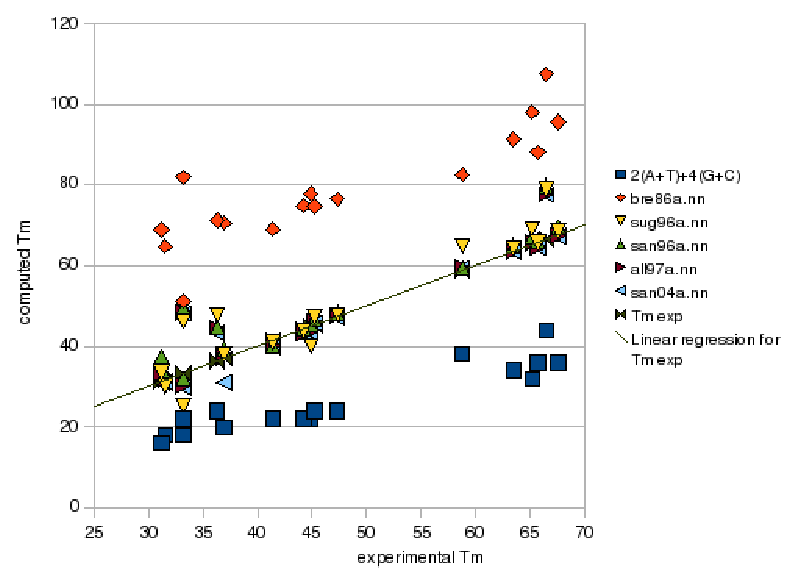
\includegraphics{image1M.eps}
\caption{Comparison of experimental and computed Tm for various sets of
  nearest-neighbor parameters. $[\mbox{Na}^+] = 1$~M, $[\mbox{nucleic acid}] = 4\cdot{}10^{-4}$~M}
\end{figure}

\begin{figure}[h]
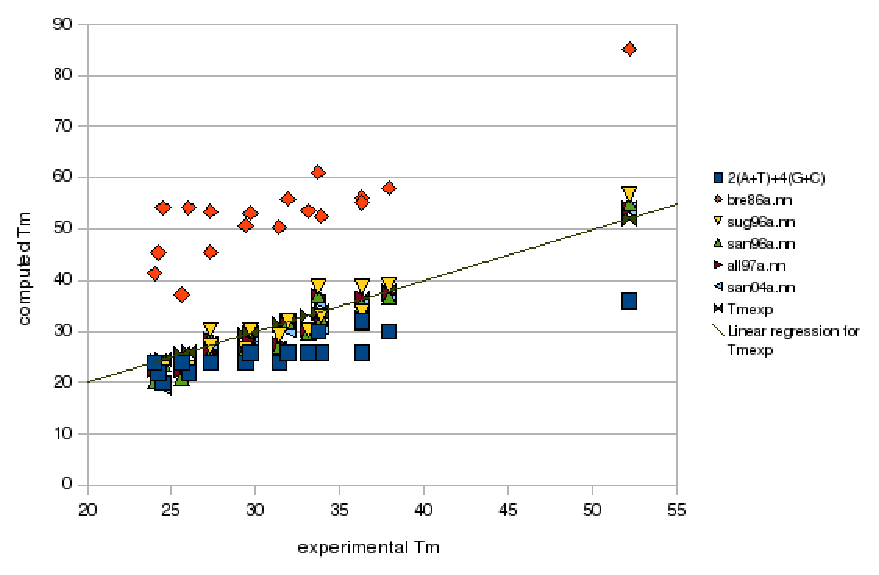
\includegraphics{image0_11M.eps}
\caption{Comparison of experimental and computed Tm for various sets of
  nearest-neighbor parameters. $[\mbox{Na}^+] = 0.11$~M, $[\mbox{nucleic acid}] = 8\cdot{}10^{-6}$~M}
\end{figure}
   
\subsection{Effect of mismatches and dangling ends}  

The mismatching pairs (inosine  mismatches  included) are also taken into account. However the thermodynamic
parameters are still not available for every possible cases (notably when both
positions are mismatched). In such a case, the program, unable to compute any
relevant result, will quit with a warning.  The two first and positions cannot
be mismatched. in such a case, the result is unpredictable, and all cases are
possible. for instance (see Allawi and SanLucia 1997), the duplex
\begin{alltt}
A          T  
 \underline{G}TGAGCTCA\underline{T}  
 \underline{T}ACTCGAGT\underline{G}  
T          A   
\end{alltt}

is more stable than 

\begin{alltt}
A\underline{G}TGAGCTCA\underline{T}T 
T\underline{T}ACTCGAGT\underline{G}A 
\end{alltt}
   
The dangling ends, that is the unmatched terminal nucleotides, can be taken into
account.

\subsection{Example}

\begin{multline*}
\Delta H {\mbox{\texttt{AGCGATGAA-}} \choose \mbox{\texttt{-CGCTGCTTT}}} = 
\Delta H {\mbox{\texttt{AG}} \choose \mbox{\texttt{-C}} } + 
\Delta H {\mbox{\texttt{A-}} \choose \mbox{\texttt{TT}} } \\ +
\Delta H {\mbox{\texttt{G}} \choose \mbox{\texttt{C}} }_\mathrm{init} +
\Delta H {\mbox{\texttt{A}} \choose \mbox{\texttt{T}} }_\mathrm{init} \\ +
\Delta H {\mbox{\texttt{GC}} \choose \mbox{\texttt{CG}} } +
\Delta H {\mbox{\texttt{CG}} \choose \mbox{\texttt{GC}} } +
2x \Delta H {\mbox{\texttt{GA}} \choose \mbox{\texttt{CT}} } +
\Delta H {\mbox{\texttt{AA}} \choose \mbox{\texttt{TT}} } \\ +
\Delta H {\mbox{\texttt{A\underline{T}}} \choose \mbox{\texttt{T\underline{G}}} } +
\Delta H {\mbox{\texttt{\underline{T}G}} \choose \mbox{\texttt{\underline{G}C}} }
\end{multline*}

       (The same computation is performed for $\Delta S$)


\subsection{The melting temperature }  
Then the melting temperature is computed by the following formula:   

\begin{tabular}{rcp{1.6in}p{2.2in}}
Tm & = & \begin{math} \frac{\Delta{}H}{\Delta{}S + R \ln (C_T/F)} \hspace{2em} + \end{math} & \begin{math}\mathcal{F}([\mathrm{Na}^+]) - 273.15 \end{math} \\
   &   &                                                                                          &                                                       \\
   &   & \footnotesize \textit{Tm} in K (for [Na$^+$] = 1~M)    &\footnotesize \emph{correction} for the 
salt concentration (if there are only Na+ cations in the solution) and to get the temperature in degree Celsius. (In fact 
some corrections are directly included in the $\Delta S$ see that of SanLucia 
1998)    
\end{tabular}
   
\subsection{Correction for the concentration of nucleic acid }  

\textit{F} is 1 in the case of self-complementarity oligonucleotides. If the
ODNs are not self-complementary, \textit{F} is 4 if both strands are present in
equivalent amount and \textit{F} is 2 if one strand is in excess (for instance
in \textsc{pcr} experiments).  Actually in the latter case, the formula would
have to use the difference of concentrations rather than the total
concentration. But if the excess is sufficient, the total concentration can be
assumed to be identical to the concentration of the strand in excess. That is,
if one strand is in excess, the actual formula is effectively $(C_{\mbox{max}} -
C_{\mbox{min}})/2$ but if $C_{\mbox{max}} \gg C_{\mbox{min}}$, $C_{\mbox{max}}
- C_{\mbox{min}}$ is close to the total concentration $C_T$.  If $C_{\mbox{max}}$ is close
to $C_{\mbox{min}}$, $(C_{\mbox{max}} - C_{\mbox{min}})/2$ is equivalent to $C_T/4$, which is the default
correction.

Note however that \textsc{melting} makes the assumption of no self-assembly,
\textit{i.e.}  the computation does not take any entropic term to correct for
self-complementarity.
  
\subsection{Correction for the concentration of salt }  

If there are only sodium ions in the solution, we can use the following
corrections:  the correction can be chosen between \textit{wet91a,} presented in
Wetmur 1991 \textit{i.e.}
\begin{displaymath}
  16.6  \log \frac{[\mbox{Na}^+]}{1 + 0.7 [\mbox{Na}^+]} + 3.85   
\end{displaymath}

  \textit{san96a} presented in SantaLucia et al. 1996 
\textit{i.e.}  
\begin{displaymath}
12.5  \log [\mbox{Na}^+]   
\end{displaymath}
  and  \textit{san98a} presented in SantaLucia 1998 \textit{i.e.} a correction 
of the entropic term without modification of enthalpy  
\begin{displaymath}
  \Delta{}S=\Delta{}S_{[\mbox{Na}^+]=1\;\mathrm{M}}+0.368 (N-1) \ln [\mbox{Na}^+]   
\end{displaymath}
  Where \emph{N} is the length of the duplex.   
   
\begin{figure}[h]
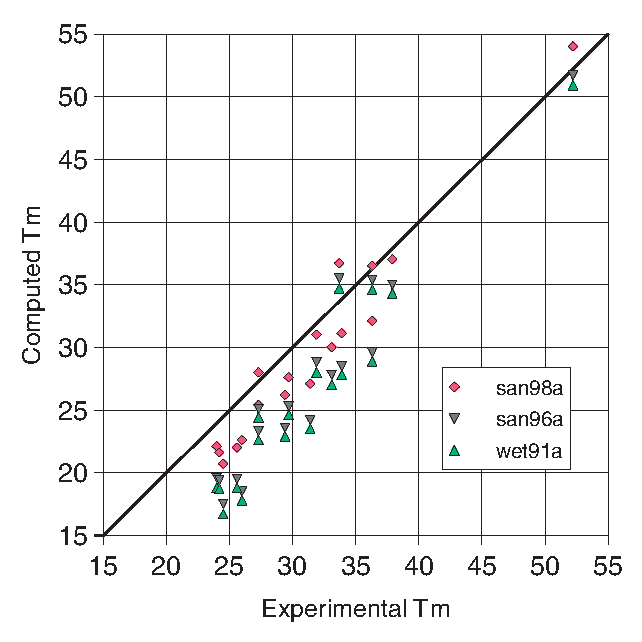
\includegraphics{salt.eps}
\caption{Comparison of experimental and computed Tm for various correction
of salt concentration.}
\end{figure}

\subsection{Correction for the concentration of ions when other monovalent ions such as 
Tris+ and K+ or divalent Mg2+ ions are added}  

If there are only Na+ ions, we can use the correction for the concentration of salt
(see above). In the opposite case, we will use the magnesium and monovalent ions correction
from Owczarzy (2008). (only for DNA duplexes)
\begin{displaymath}
 [\mbox{Mon}^+] = [\mbox{Na}^+] + [\mbox{k}^+] + [\mbox{Tris}^+]
\end{displaymath}
  Where $[\mbox{Tris}^+]$ is equal to half of total tris buffer concentration. (in the option -t, it is the Tris buffer concentration
which is entered).

When the divalent ions are the only ions present, the melting temperature is :
\begin{displaymath}
\frac{1}{Tm_{[\mbox{Mg}^{2+}]}} = \frac{1}{Tm_{[\mbox{Na}^+]=1\;\mathrm{M}}} + a
- b (\ln [\mbox{Mg}^{2+}]) + Fgc (c + d \ln [\mbox{Mg}^{2+}]) + \frac{1}{2 (Nbp-1)} 
\end{displaymath}
\begin{displaymath}
(-e + f \ln [\mbox{Mg}^{2+}] + g (\ln [\mbox{Mg}^{2+}])^{2}])
\end{displaymath}
   where : 
a = 3.92 x $10^{-5}$
b = 9.11 x $10^{-6}$
c = 6.26 x $10^{-5}$
d = 1.42 x $10^{-5}$
e = 4.82 x $10^{-4}$
f = 5.25 x $10^{-4}$
g = 8.31 x $10^{-5}$.

Fgc is the fraction of GC base pairs in the sequence and 
Nbp is the length of the sequence (Number of base pairs).

When there are both monovalent and divalent ions, there are several cases because we can have
a competitive DNA binding between monovalent and divalent 
cations.

If the following ratio :
\begin{displaymath}
  \frac{[\mbox{Mg}^{2+}]^{0.5}]}{[\mbox{Mon}^+]}  
\end{displaymath}
is inferior to 0.22, monovalent ion influence is dominant, divalent cations can be 
disregarded and the melting temperature is :
\begin{displaymath}
\frac{1}{Tm_{[\mbox{Mg}^{2+}]}} = \frac{1}{Tm_{[\mbox{Na}^+]=1\;\mathrm{M}}} + (4.29
Fgc - 3.95)\cdot{}10^{-5} \ln [\mbox{Mon}^+] + 9.40\cdot{}10^{-6} (\ln [\mbox{Mg}^{2+}])^{2})
\end{displaymath}
  
\begin{figure}[H]
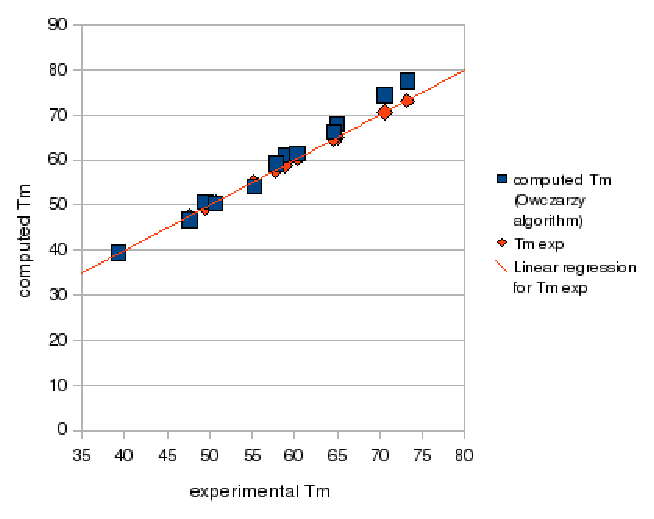
\includegraphics{Owczarzy2.eps}
\caption{Comparison of experimental and computed Tm with the algorithm published
in Owczarzy et al (2008). $[\mbox{Mon}^+] = 0.055$~M, $[\mbox{Mg}^{2+}] = 0$~M, $[\mbox{nucleic acid}] =
2\cdot{}10^{-6}$~M. The ratio is inferior to 0.22}
\end{figure}


If the ratio is included in [0.22, 6[,we must take in account both Mg2+ and monovalent cations 
concentrations. The melting temperature is calculated with the first equation but with monovalent 
ions concentration dependent parameters a, d and g :

\begin{displaymath}
a = 3.92\cdot{}10^{-5} (0.843 - 0.352 [\mbox{Mon}^+]^{0.5} \ln [\mbox{Mon}^+]) 
\end{displaymath}
\begin{displaymath}
d = 1.42\cdot{}10^{-5} (1.279 - 4.03\cdot{}10^{-3} \ln [\mbox{Mon}^+] -
8.03\cdot{}10^{-3} \ln [\mbox{Mon}^+]^{2})
\end{displaymath}
\begin{displaymath}
g = 8.31\cdot{}10^{-5} (0.486 - 0.258 \ln [\mbox{Mon}^+] + 5.25\cdot{}10^{-3}
\ln [\mbox{Mon}^+]^{3} 
\end{displaymath}

\begin{figure}[H]
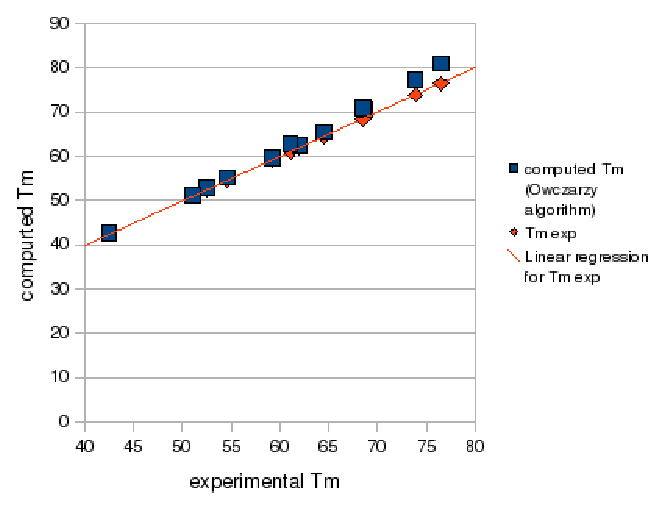
\includegraphics{Owczarzy3.eps}
\caption{Comparison of experimental and computed Tm with the algorithm published
in Owczarzy et al (2008). $[\mbox{Mon}^+] = 0.055$~M, $[\mbox{Mg}^{2+}] = 0.0015$~M, $[\mbox{nucleic acid}] =
2\cdot{}10^{-6}$~M. The ratio is included in [0.22, 6[.}
\end{figure}

Finally, if the ratio is superior to 6,divalent ion influence is dominant, monovalent cations can be 
disregarded and the melting temperature is calculated with the first equation and the constant parameters a, b, c, d,
e, f, g.

\begin{figure}[H]
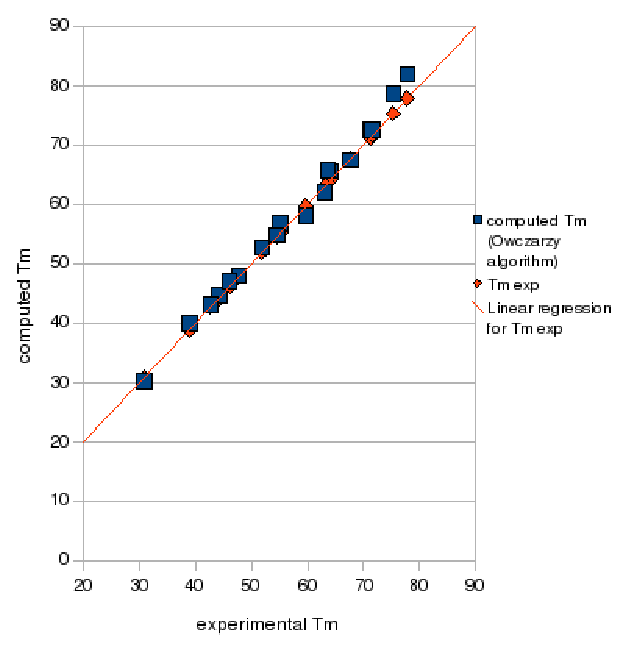
\includegraphics{Owczarzy1.eps}
\caption{Comparison of experimental and computed Tm with the algorithm published
in Owczarzy et al(2008). $[\mbox{Mon}^+] = 0.001$~M, $[\mbox{Mg}^{2+}] = 0.0015$~M, $[\mbox{nucleic acid}] =
2\cdot{}10^{-6}$~M. The ratio is superior to 6.}
\end{figure}
    
\subsection{Long sequences }  
  It is important to realise that the nearest-neighbor approach 
has been established  on small oligonucleotides. Therefore the use of \textsc{melting} 
in the non-approximative  mode is really accurate only for relatively short 
sequences (Although if the sequences are two short, let's say $<$ 6~bp, the 
influence of extremities becomes too important and the  reliability decreases 
a lot). For long sequences an approximative mode has been designed. This mode is 
launched if the sequence length is higher than the value 
given by the option -T (the default threshold is 60 bp).
 
The melting temperature is computed by the following formulas:   

\textsc{adn/adn}:
\begin{displaymath}
Tm = 81.5 + 16.6\log\frac{[\mbox{Na}^+]}{1+0.7[\mbox{Na}^+]} + 0.41\% GC - \frac{500}{size}
\end{displaymath}
\textsc{adn/arn}:
\begin{displaymath}
Tm = 67 + 16.6\log\frac{[\mbox{Na}^+]}{1+0.7[\mbox{Na}^+]} + 0.8\% GC - \frac{500}{size}
\end{displaymath}
\textsc{arn/arn}:
\begin{displaymath}
Tm = 78 + 16.6\log\frac{[\mbox{Na}^+]}{1+0.7[\mbox{Na}^+]} + 0.7\% GC - \frac{500}{size}
\end{displaymath}

  The usage of this mode is nevertheless  \textbf{strongly disencouraged.}   
   
\subsection{Miscellaneous comments }  
\textsc{melting} is currently accurate only when the hybridisation is performed
at pH $7\pm 1$.  The computation is valid only for the hybridisations performed
in aqueous medium. Therefore the use of denaturing agents such as formamide
completely invalidates the results.
   
\section{References }
Allawi 
H.T., SantaLucia J. (1997). Thermodynamics and NMR of internal G-T mismatches 
in DNA. \textit{Biochemistry}  36: 10581-10594   

Allawi H.T., SantaLucia J. (1998). Nearest Neighbor thermodynamics parameters 
for internal G.A mismatches in DNA. \textit{Biochemistry} 37: 2170-2179

Allawi H.T., SantaLucia J. (1998).Thermodynamics of internal C.T mismatches in DNA.
\textit{Biochemistry} 26: 2694-2701.

Allawi H.T., SantaLucia J. (1998). Nearest Neighbor thermodynamics of internal 
A.C mismatches in DNA: sequence dependence and pH effects.
\textit{Biochemistry} 37: 9435-9444.

Bommarito S., Peyret N., SantaLucia J. (2000).  Thermodynamic parameters for DNA
sequences with dangling ends.  \textit{Nucleic Acids Res} 28: 1929-1934

  Breslauer K.J., Frank R., Bl\"ocker 
H., Marky L.A. (1986). Predicting DNA duplex stability from the base sequence. 
 \textit{Proc Natl Acad Sci USA}  83: 3746-3750   

  Freier S.M., Kierzek R., Jaeger 
J.A., Sugimoto N., Caruthers M.H., Neilson T., Turner D.H. (1986). \textit{Biochemistry} 
 83:9373-9377 
 
 Owczarzy R., Moreira B.G., You Y., Behlke M.B., Walder J.A.(2008) Predicting stability of DNA duplexes 
 in solutions containing Magnesium and Monovalent Cations. \textit{Biochemistry} 47: 5336-5353.  

Peyret N., Seneviratne P.A., Allawi H.T., SantaLucia J. (1999). Nearest Neighbor thermodynamics and 
NMR of DNA sequences with internal A.A, C.C, G.G and T.T mismatches. dependence and pH effects.
\textit{Biochemistry} 38: 3468-3477

  SantaLucia J. Jr, Allawi H.T., Seneviratne P.A. (1996). Improved 
nearest-neighbor parameters for predicting DNA duplex stability. \textit{Biochemistry} 
35: 3555-3562   

  Sugimoto N., Katoh M., Nakano S., Ohmichi T., Sasaki M. (1994). 
RNA/DNA hybrid duplexes with identical nearest-neighbor base-pairs hve identical 
stability. \textit{FEBS Letters} 354: 74-78   

  Sugimoto N., Nakano S., Katoh M., Matsumura 
A., Nakamuta H., Ohmichi T., Yoneyama M., Sasaki M. (1995). Thermodynamic parameters 
to predict stability of RNA/DNA hybrid duplexes. \textit{Biochemistry} 34: 11211-11216 
  
  Sugimoto N., Nakano S., Yoneyama M., Honda K. (1996).  Improved thermodynamic 
parameters and helix initiation factor to predict stability of DNA duplexes. 
\textit{Nuc Acids Res}  24: 4501-4505  

Watkins N.E., Santalucia J. Jr. (2005). Nearest-neighbor thermodynamics of deoxyinosine 
pairs in DNA duplexes. \textit{Nuc Acids Res} 33: 6258-6267 

Wright D.J., Rice J.L., Yanker D.M., Znosko B.M. (2007). Nearest neighbor parameters for 
inosine-uridine pairs in RNA duplexes. \textit{Biochemistry} 46: 4625-4634

  Xia T., SantaLucia J., Burkard M.E., Kierzek 
R., Schroeder S.J., Jiao X., Cox C., Turner D.H. (1998). Thermodynamics parameters 
for an expanded nearest-neighbor model for formation of RNA duplexes with 
Watson-Crick base pairs. \textit{Biochemistry}  37: 14719-14735   

  For review see: 
  
  SantaLucia J. (1998) A unified view of polymer, dumbbell, and oligonucleotide 
DNA nearest-neighbor thermodynamics. \textit{Proc Natl Acad Sci USA}  95: 1460-1465 

SantaLucia  J., Hicks Donald (2004) The Thermodynamics of DNA structural motifs. 
\textit{Annu. Rev. Biophys. Struct} 33: 415-440 
  
  Wetmur J.G. (1991) DNA probes: applications of the principles of nucleic 
acid hybridization. \textit{Crit Rev Biochem Mol Biol} 26: 227-259   
   
\section{Files }
\begin{itemize}
\item [\textit{*.nn}] Files containing the nearest-neighbor parameters, enthalpy and entropy, 
for each Crick's pair.  They have to be placed in a directory defined during 
the compilation or targeted by the  environment variable NN\_PATH.  
\item [\textit{tkmelting.pl}] A Graphical User Interface written in perl/tk is available for users
who prefer  the 'button and menu' approach.  
\item [\textit{*.pl}] Scripts are available to 
use \textsc{melting} iteratively. For instance, the script multi.pl permits to predict 
the Tm of several duplexes in one shot. The script profil.pl allow
an interactive computation along a sequence, by sliding a window of specified width. 
  
\end{itemize}
 
\section{See Also }
New versions and 
related material can be found at \url{http://www.pasteur.fr/recherche/unites/neubiomol/meltinghome.html} 
and at \url{https://sourceforge.net/projects/melting/}
  
You can use \textsc{melting} through a web server at \url{http://bioweb.pasteur.fr/seqana
l/interfaces/melting.html}
  
\section{Known Bugs }
The infiles have to be ended by a blank line because otherwise the last line is not decoded.

If an infile is called, containing the 
address of another input file, it does not care of this latter.  If it 
is its own address, the program quit (is it a bug or a feature?).   
 
In interactive mode, a sequence can be entered on several lines with a backslash\\
\texttt{AGCGACGAGCTAGCCTA{\textbackslash}\\
AGGACCTATACGAC}\\
If by mistake it is entered as  \\
\texttt{AGCGACGAGCTAGCCTA{\textbackslash}{}AGGACCTATACGAC}

The backslash will be considered 
 as an illegal character. Here again, I do not think it is actually a bug 
(even if it is unlikely, there is a small probability that the  backslash 
could actually be a mistyped base).   
   
\section{Copyright }
Melting is copyright 
\copyright 1997, 2009 by Nicolas Le Nov\`ere and Marine Dumousseau.  

This program is free software; 
you can redistribute it and/or modify it under the terms of the GNU General 
Public License as published by the Free Software Foundation; either version 
2 of the License, or (at your option) any later version.   
  This program 
is distributed in the hope that it will be useful, but WITHOUT ANY WARRANTY; 
without even the implied warranty of MERCHANTABILITY or FITNESS FOR A 
PARTICULAR PURPOSE.  See the GNU General Public License for more details. 
  
  You should have received a copy of the GNU General Public License 
along with this program; if not, write to the Free Software Foundation, 
Inc., 59 Temple Place, Suite 330, Boston, MA  02111-1307 USA   
   
\section{Acknowledgements}
Nicolas Joly is an efficient and kind debugger and advisor.  Catherine
Letondal wrote the HTML interface to melting. Thanks to Nirav Merchant,
Taejoon Kwon, Leo Schalkwyk, Mauro Petrillo, Andrew Thompson, Wong Chee Hong, Ivano
Zara for their bug fixes and comments. Thanks to Richard Owczarzy for his magnesium 
correction. Thanks to Charles Plessy for the graphical interface files. Finally thanks
to the usenet helpers, particularly Olivier Dehon and Nicolas Chuche.

   
\section{Authors }
Nicolas Le Nov\`ere and Marine Dumousseau, \\
EMBL-EBI, 
Wellcome-Trust Genome Campus
Hinxton Cambridge, CB10 1SD, UK
lenov@ebi.ac.uk
  
\section{History }

See the file ChangeLog for the changes of the versions 4 and more recent.

\end{document}
